% Permission is granted to copy, distribute and/or modify this
% document under the terms of the Creative Common by-nc-sa License
% version 3.0 (CC BY-NC-SA 3.0). A copy of the license can be found at
% http://creativecommons.org/licenses/by-nc-sa/3.0/legalcode.
%

%% Slides Class
\documentclass[10pt,a4paper]{beamer}

%% Setting beamer style
\usepackage{UBdx}

\setbeamertemplate{bibliography entry title}{}
\setbeamertemplate{bibliography entry location}{}
\setbeamertemplate{bibliography entry note}{}

%% Font packages
\usepackage{lmodern}
\usepackage[T1]{fontenc}
\usepackage[utf8]{inputenc}
\usepackage{babel}
\usepackage[colorinlistoftodos]{todonotes}
\usepackage{listings}
\usepackage{amssymb}
\usepackage{amsmath}
\usepackage{amsthm}
\usepackage{appendix}
\usepackage{multicol}
\usepackage{stmaryrd}
\usepackage{verbatim}
\usepackage{algorithm, algorithmic}

\theoremstyle{plain}
\newtheorem{thm}{Théorème}[section]
\newtheorem{lemme}[thm]{Lemme}
\newtheorem{propo}[thm]{Proposition}

\theoremstyle{definition}
\newtheorem{remarque}[thm]{Remarque}
\newtheorem{defi}[thm]{Définition}
\newtheorem{nota}[thm]{Notation}


\renewcommand{\a}{\alpha}
\newcommand{\HRule}{\rule{\linewidth}{0.5mm}} 
\newcommand{\F}{\mathbb{F}} 
\newcommand{\A}{\mathcal{A}} 
\newcommand{\e}{\mathbf{e}}  
\newcommand{\s}{\mathbf{s}} 
\newcommand{\K}{\mathbb{K}} 
\newcommand{\J}{\mathcal{J}} 
\newcommand{\D}{\mathcal{D}} 

% traduction des mots pour les algos
\floatname{algorithm}{Algorithme}
\renewcommand{\algorithmicrequire}{\textbf{Entrées:}}
\renewcommand{\algorithmicensure}{\textbf{Sortie:}}
\renewcommand{\algorithmicrepeat}{\textbf{Faire}}
\renewcommand{\algorithmicuntil}{\textbf{Tant que}}
\renewcommand{\algorithmicreturn}{\textbf{Retourne}}

% Highlight macros
\newcommand{\highlight}[1]{\textcolor{structure.fg}{\bfseries #1}}

%% Title, subtitle, authors, institute, date, ...
\title{Projet - Wave}
\subtitle{Un procédé de signature à base de codes correcteurs}
\author{ Suzanne LANSADE, Eva PALANDJIAN \\\quad\quad\quad\quad\quad \\Encadrant : Gilles ZEMOR}


\institute[Master CSI]{Master CSI, Université de Bordeaux, France}

\date{25 Février 2020}

%%%%%%%%%%%%%%%%%%%%%%%%%%[ Document ]%%%%%%%%%%%%%%%%%%%%%%%%%%
\begin{document}

\begin{frame}
  \vspace{3.5em}
  \titlepage

\end{frame}

\begin{frame}
  \frametitle{Plan}
  \tableofcontents[subsectionstyle=hide]
\end{frame}

%%%%%%%%%%%%%%%%%%%%%%%%%%%%%%%%%%%%%%%%%%%%%%%%%%%%%%%%%%%%%%%%%%%
\section{Introduction}
\begin{frame}
\frametitle{Introduction}
\begin{itemize}
\item[•] Éventualité de l'arrivée de l'ordinateur quantique:
       \begin{itemize}
       \item[$\rightarrow$] On cherche des alternatives à RSA et DH 
       \item[$\rightarrow$] Le NIST lance en 2017 un appel pour la standardisation des systèmes à clef publique
       \end{itemize}
\vspace{0.2in}
\item[•] Les codes correcteurs
       \begin{itemize}
       \item[$\rightarrow$] Peuvent être quantiquement
        sûrs
       \item[$\rightarrow$] Peuvent déjà être utilisés dans des systèmes de chiffrement
       \item[$\rightarrow$] Sont difficilement utilisables pour les signatures
       \end{itemize}
\end{itemize}
\end{frame}

\begin{frame}
\frametitle{Introduction}
\begin{figure}[h]
\begin{center}
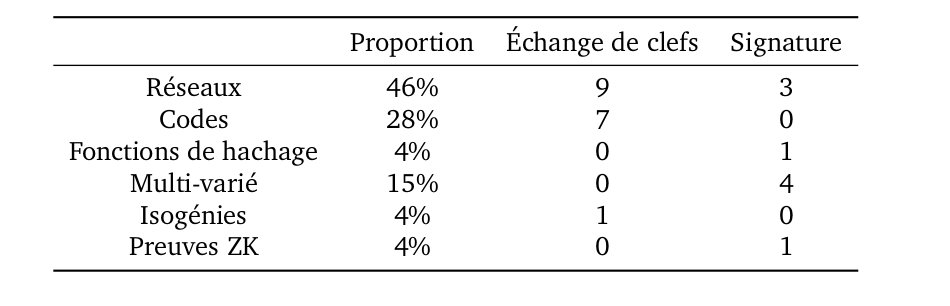
\includegraphics [scale=0.3]{../rapport/include/nist_second_tour.png}
\end{center}
\caption{\small Comparaison des soumissions au NIST du second tour.}
\end{figure}
\end{frame}

\begin{frame}
\frametitle{Introduction}
\begin{itemize}    
\item[•] Difficile de faire un système de signature à base de codes 
       \begin{itemize}
       \item[$\rightarrow$] Difficile de se placer dans l'ensemble des syndromes facilement et \\uniquement décodables
       \item[$\rightarrow$] Tous les systèmes existant sont cassés ou inutilisables dans la pratique
       \end{itemize}
\vspace{0.2in}
\item[•] Le système Wave
       \begin{itemize}
       \item[$\rightarrow$] Enlève la restriction au mot le plus proche
       \item[$\rightarrow$]Décode en grande distance
       \end{itemize}
\end{itemize}   

\end{frame}

%%%%%%%%%%%%%%%%%%%%%%%%%%%%%%%%%%%%%%%%%%%%%%%%%%%%%%%%%%%%%%%%%%%%%%
\section{Schéma de signature Wave}
\begin{frame}
  \frametitle{Plan}
  \tableofcontents[currentsection,subsectionstyle=hide]
\end{frame}

\subsection{Codes $(U,U+V)$-généralisés}

\begin{frame}
\frametitle{Codes $(U,U+V)$-généralisés} 

Le système de signature Wave utilise une famille de codes correcteurs appelés codes $(U,U+V)$-généralisés.
\vspace{0.15in}
\begin{block}{}
Soit $n$ un entier pair, et soient $U$ et $V$ deux codes aléatoires de dimension respectives $k_U$ et $k_V$ et de longueur $n/2$. Le \textit{code $(U,U+V)$-généralisé } correspond à l'ensemble des mots :
\begin{center}
$ \{(a.u + b.v, c.u + d.v)$ tel que $u \in U$ et $v \in V \}$
\end{center}
\vspace{0.1in}
où $x.y$ est le produit coordonnée par coordonnée des $x_i$ et $y_i$ et $a$,$b$,$c$,$d$ sont quatre vecteurs de $\F_q^{n/2}$.
\end{block}
\end{frame}


\subsection{Signature}

\begin{frame}[fragile]
\frametitle{Signature}
\begin{itemize}
\item[•]  Le système Wave utilise la fonction qui a un vecteur $\e$ de poids $\omega$\\ associe son syndrome par $\mathbf{H}$ :
$$ f_{\omega,\mathbf{H}}: \e \longrightarrow \e H^T = s $$
comme fonction à sens unique
\vspace{0.2in}
\item[•]  Il utilise un algorithme \verb|InvertAlg| permettant d'inverser la fonction syndrome à l'aide de la trappe $T$
\vspace{0.2in}
\item[•]  La trappe $T$ correspond à la structure du code $(U,U+V)$-généralisé
\end{itemize}
\end{frame}

\begin{frame}[fragile]
\frametitle{Signature}
Le schéma de signature Wave est donc composé de deux algorithmes :
 \begin{columns}[t]
  \begin{column}{5cm}
  \begin{block}{}
    $\verb|Sign|^{sk}(s)$:\\
	$\quad \;\e \leftarrow  \verb|InvertAlg|(s,T)$ \\
 	$\quad \verb| renvoie | \e$
  \end{block} 
  \end{column}
  
  \begin{column}{5cm}
  \begin{block}{}
    $\verb|Verify|^{pk}(s,e')$: \\
	$\quad \verb| Si | \e'H^T = s \verb| et | |\e'| = \omega $ \\
	$\quad \quad \verb| renvoie 1| $\\
	$\quad \verb| renvoie 0|$
  \end{block}   
  \end{column}
 \end{columns}  
 
\vspace{0.2in}
\begin{itemize}
\item[•] L'algorithme de signature utilise la trappe et un algorithme de décodage \\pour renvoyer une erreur de poids $\omega$
 \vspace{0.1in}
\item[•] L'algorithme de vérification accepte la signature si le syndrome et le poids sont corrects 
\end{itemize}
\end{frame}

\subsection{Décodage}

\begin{frame}
\frametitle{Décodage}
Soit 

$$\begin{array}{ccccc}
\varphi_{\mathbf{a},\mathbf{b},\mathbf{c},\mathbf{d}} & : & \F_q^{n/2} \times  \F_q^{n/2} & \to & \F_q^{n/2} \times  \F_q^{n/2} \\
 & & (\mathbf{x} , \mathbf{y}) & \mapsto &  (a.\mathbf{x} + b.\mathbf{y}, c.\mathbf{x} + d.\mathbf{y}) \\
\end{array}$$


\begin{propo} Inverser $f_{\omega,\mathbf{H}}$ pour un certain $\mathbf{s} \in F_q^{n-k}$ est équivalent à trouver $\mathbf{e} \in \F_q^n$ tel que:
$$ \mathbf{e}_U\mathbf{H}_U^T = \mathbf{s}^U \qquad \text{et} \qquad \mathbf{e}_V\mathbf{H}_V^T = \mathbf{s}^V $$

\vspace{0.1in}
où $\mathbf{s} = (\mathbf{s}^U, \mathbf{s}^V)$ avec $\mathbf{s}^U \in \F_q^{n/2-k_U}$, $\mathbf{s}^V \in \F_q^{n/2-k_V}$ et où
$\mathbf{e}_U$ et $\mathbf{e}_V$ de $\F_q^{n/2}$ sont\\
\vspace{0.1in}
tels que $(\mathbf{e}_U,\mathbf{e}_V) = \varphi^{-1}_{a,b,c,d}(\mathbf{e}).$
\end{propo}
\end{frame}

\begin{frame}
\frametitle{Décodage}
\begin{figure}
\begin{center}
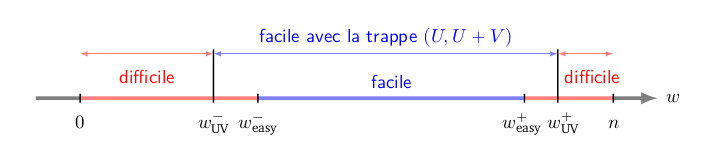
\includegraphics [scale=0.4]{schema.png}
\end{center}
\end{figure}

\vspace{0.2in}

\begin{itemize}
\item[•] On veut se placer dans un intervalle qui permet de décoder, mais uniquement en connaissant la trappe
\vspace{0.1in}
\item[•] On prend $\omega \in \llbracket \omega_{easy}^+, \omega_{UV}^+\rrbracket$
\vspace{0.1in}
\item[•] Afin d'obtenir une erreur de poids $\omega$ on pose des contraintes sur le vecteur $\e_U$
\end{itemize}

\end{frame}

\begin{frame}
\frametitle{Décodage}

\vspace{0.15in}
\begin{block}{}
Pour tout $\mathbf{e} = \varphi_{\mathbf{a},\mathbf{b},\mathbf{c},\mathbf{d}}(\mathbf{e_U},\mathbf{e_V})$, on a pour tout $i \in \llbracket 1,n/2\rrbracket$ :

\begin{center}
$\left \{
\begin{array}{rcl}
a_i\mathbf{e}_U(i) + b_i\mathbf{e}_V(i) &=& \mathbf{e}(i) \\[0.3cm]
c_i\mathbf{e}_U(i) + d_i\mathbf{e}_V(i) &=& \mathbf{e}(i+n/2) 
\end{array}
\right.$
\end{center}
\end{block}

\vspace{0.1in}

\begin{itemize}
\item[•] On décode $\e_U$ avec une variante du décodage par ensemble d'information
\vspace{0.1in}
\item[•] On choisi $k_U$ coordonnées de $\e_U$ telles que les lignes du système soient non nulles à ces positions
\vspace{0.1in}
\item[•] Ainsi on aura
	\begin{itemize}
	\vspace{0.05in}
	\item[$\rightarrow$] $2k_U$ coordonnées de $\e$ non nulles
	\vspace{0.1in}
	\item[$\rightarrow$] Les $n-2k_U$ autres seront uniformément distribuées dans leur ensemble
	\end{itemize}
\end{itemize}

\end{frame}

\begin{frame}
\frametitle{Décodage}
\begin{figure}[h]
\begin{center}
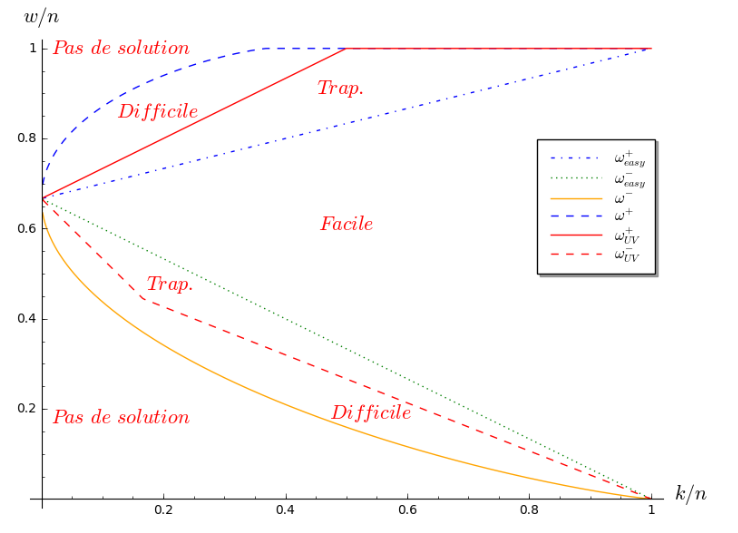
\includegraphics [scale=0.32]{../rapport/include/graph_ratio_w.png}
\end{center}
\caption{\scriptsize Comparaison des distances $w/n$ avec et sans trappe en fonction du rendement.}
\end{figure}
\end{frame}

%%%%%%%%%%%%%%%%%%%%%%%%%%%%%%%%%%%%%%%%%%%%%%%%%%%%%%%%%%%%%%%%%%%%%%
\section{Uniformisation des sorties}

\begin{frame}
  \frametitle{Plan}
  \tableofcontents[currentsection,subsectionstyle=hide]
\end{frame}

\begin{frame}
\frametitle{Uniformisation des sorties}

\begin{itemize}
\item[•] Des corrélations vont apparaître entre les coordonnées $\e_i$ et $\e_{i+n/2}$
\vspace{0.05in}
	\begin{itemize}
	\item[$\rightarrow$] Si un attaquant $\mathcal{A}$ récupère suffisamment de signatures, il pourra calculer :
$$\mathbb{P}(\mathbf{e}_i \neq \mathbf{e}_{i+n/2})\quad \text{et}\quad\mathbb{P}(\mathbf{e}_i \neq \mathbf{e}_{j})\qquad\qquad\qquad\qquad\qquad\qquad\qquad\qquad\qquad\qquad$$
	\end{itemize}
	
\vspace{0.3in}
\item[•] Normalement les coordonnées de $\e$ sont permutées pour cacher la structure du code
\vspace{0.05in}
	\begin{itemize}
	\item[$\rightarrow$] $\mathcal{A}$ peut donc retrouver la permutation
	\end{itemize}
\end{itemize}

\end{frame}

\begin{frame}[fragile]
\frametitle{La méthode du rejet}
\vspace{-0.3in}
\begin{figure}[h]
\begin{center}
\includegraphics [scale=0.38]{algo_uv.png}
\end{center}
\end{figure}
$$ \text{Où  } m_1(x) := \# \; \{1  \leq i \leq n/2 \;;\; |(x_i, x_{i+n/2})| = 1\}$$
\end{frame}


\begin{frame}
\frametitle{La méthode du rejet}
\begin{figure}[h]
\begin{center}
\includegraphics [scale=0.35]{decodeV.png}
\end{center}
\end{figure}

\vspace{-0.1in}

\begin{figure}[h]
\begin{center}
\includegraphics [scale=0.35]{decodeU.png}
\end{center}
\end{figure}
\end{frame}

\begin{frame}
\frametitle{La méthode du rejet}
Soient $X$ et $X^{unif}$ deux variables aléatoires à valeur dans un même ensemble $\mathcal{X}$.
Pour tout $x \in \mathcal{X}$ on pose :
\begin{equation*}
    r(x) := \left(\inf\limits_{y \in \mathcal{X}}\frac{\mathbb{P}(X=y)}{\mathbb{P}(X^{unif}=y)}\right) \frac{\mathbb{P}(X^{unif}=x)}{\mathbb{P}(X=x)}
\end{equation*}
\vspace{0.2in}
Soit la variable aléatoire $Y$ définie telle que :
\begin{enumerate}
\item[1.] On tire $x \in \mathcal{X}$ selon la distribution $X$
\vspace{0.1in}
\item[2.] On tire $\theta$ uniformément dans l'intervalle $\llbracket 0,1 \rrbracket$
\vspace{0.1in}
\item[3.] Si $\;\theta \leq r(x)$, alors $Y$ prend la valeur $x$
\vspace{0.1in}
\item[4.] Sinon, on recommence
\end{enumerate}
\vspace{0.2in}
Alors $Y$ suit une loi uniforme. 

\end{frame}

\begin{frame}[fragile]
\frametitle{La méthode du rejet}
\vspace{-0.3in}
\begin{figure}[h]
\begin{center}
\includegraphics [scale=0.38]{algo_uv.png}
\end{center}
\end{figure}
$$ \text{Où  } m_1(x) := \# \; \{1  \leq i \leq n/2 \;;\; |(x_i, x_{i+n/2})| = 1\}$$
\end{frame}


%%%%%%%%%%%%%%%%%%%%%%%%%%%%%%%%%%%%%%%%%%%%%%%%%%%%%%%%%%%%%%%%%%%%%%
\section{Sécurité EUF-CMA}

\begin{frame}
  \frametitle{Plan}
  \tableofcontents[currentsection,subsectionstyle=hide]
\end{frame}

\begin{frame}[fragile]
\frametitle{Jeu EUF-CMA}	
\begin{figure}[h]
		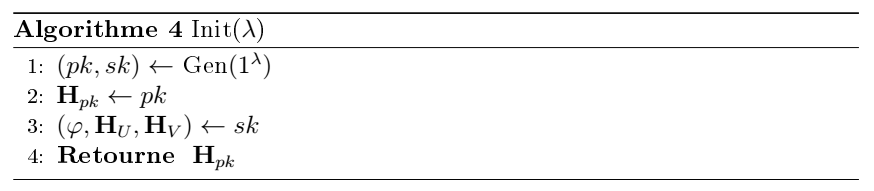
\includegraphics[width=\textwidth]{init.png}
\end{figure}

\vspace{0.1in}

L'attaquant $\mathcal{A}$ appelle la fonction \verb|Init| et récupère la matrice de parité $\mathbf{H}_{pk}$ du code $(U,U+V)$-généralisé.
\end{frame}


\begin{frame}[fragile]
\frametitle{Jeu EUF-CMA}	
\begin{figure}[h]
		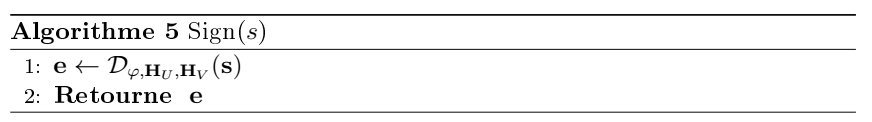
\includegraphics[width=\textwidth]{sign.png}
\end{figure}

\vspace{0.1in}

\begin{itemize}
\item[•] L'attaquant $\mathcal{A}$ peut faire $N_{sign}$ appels à la fonction \verb|Sign| et récupérer $N_{sign}$ couples $(s,\e)$
\vspace{0.1in}
\item[•] Il doit alors renvoyer un nouveau couple $(s,\e)$ où $s$ n'a jamais été demandé \\à la fonction \verb|Sign|
\end{itemize}

\end{frame}

\begin{frame}[fragile]
\frametitle{Jeu EUF-CMA}	
\begin{figure}[h]
		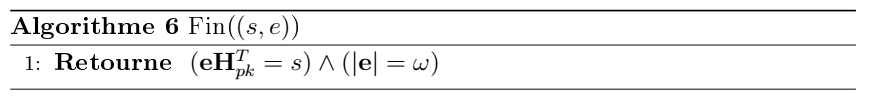
\includegraphics[width=\textwidth]{fin.png}
\end{figure}

\vspace{0.1in}

\begin{itemize}
\item[•] La fonction \verb|Fin| vérifie la validité de la signature
\vspace{0.1in}
\item[•] L'attaquant $\mathcal{A}$ a réussi le jeu EUF-CMA si la fonction \verb|Fin| renvoie 1
\end{itemize}
\end{frame}

\begin{frame}[fragile]
\frametitle{Sécurité EUF-CMA}
\begin{block}{}
On définit alors le succès EUF-CMA comme :
$$Succ^{EUF-CMA}_{Wave}(N_{sign}) := \max_{\mathcal{A}}(\mathbb{P}(\mathcal{A}\text{ réussit le jeu EUF-CMA de Wave})).$$
\end{block}	
\vspace{0.2in}
Le protocole est alors sûr au sens EUF-CMA si ce succès est négligeable. \\
\vspace{0.2in}
Pour montrer que le schéma Wave est sûr au sens EUF-CMA, nous pouvons le réduire au problème DOOM.\\
\end{frame}

\begin{frame}
\frametitle{Réduction au problème DOOM}

\begin{block}{}
\textbf{Le problème DOOM.} Soient des paramètres $(n,q,k,\omega,N)$, où $N$ est un entier. \\

\leftskip=1cm
\noindent \textbf{I :} $\mathbf{H}$ une matrice uniforme de $\F_q^{(n-k)\times n}$ et $(\mathbf{s}_1,...,\mathbf{s}_N)$ une liste de $N$ syndromes. 

\noindent \textbf{Q :} Décoder l'un des syndromes à la distance $\omega$. \\

\leftskip=0cm
\end{block}

\vspace{0.2in}
$$Succ^{DOOM} :=
 \max_{\mathcal{A}}\left[\mathbb{P}\left(\mathcal{A}(\mathbf{H},\mathbf{s}_1,...,\mathbf{s}_n)=\mathbf{e} \; \left| \; \exists  j \in \{1,...,N\} \text{ tq } \mathbf{eH}^T = \mathbf{s}_j\right)\right]\right..$$

\end{frame}




%%%%%%%%%%%%%%%%%%%%%%%%%%%%%%%%%%%%%%%%%%%%%%%%%%%%%%%%%%%%%%%%%%%%%%
\section{Implémentation}

\begin{frame}
  \frametitle{Plan}
  \tableofcontents[currentsection,subsectionstyle=hide]
\end{frame}

\begin{frame}
\frametitle{Implémentation et résultats}
\frametitle{Résultats de notre implémentation}
\begin{center}
\begin{tabular}{|c|c|c|c|} 
\hline
\textbf{nombre d'itérations} & \textbf{d} & \textbf{nombre de rejets} & \textbf{ratio\;} \\\hline 
100 & 0 & 6 & 6\% \\\hline
100 & 1 & 3 & 3\% \\\hline 
100 & 2 & 6 & 6\% \\\hline
100 & 3 & 3 & 3\% \\\hline
100 & 4 & 6 & 6\% \\\hline
100 & 5 & 4 & 4\% \\\hline
\end{tabular}
\end{center}
\begin{center}
\begin{tabular}{|c|c|c|c|} 
\hline
\textbf{nombre d'itérations} & \textbf{d} & \textbf{nombres de rejets} & \textbf{ratio} \\\hline 
400 & 3 & 19 & $\sim$5\% \\\hline
400 & 5 & 17 & $\sim$4\%\\\hline 
\end{tabular}\

\vspace{0.2in}
\textbf{Ratio moyen de l'article : $\sim$10\%}
\end{center}
\end{frame}


%%%%%%%%%%%%%%%%%%%%%%%%%%%%%%%%%%%%%%%%%%%%%%%%%%%%%%%%%%%%%%%%%%%%%%
\section*{Références}

%\begin{frame}<handout:0>
%  \frametitle{Plan}
%  \tableofcontents[currentsection,subsectionstyle=hide]
%\end{frame}



\begin{frame}
  \frametitle{Références}
  \begin{enumerate}
  \item[{[1]}] Thomas Debris-Alazard. \textit{Cryptographie fondée sur les codes : nouvelles approches pour constructions et preuves ; contribution en cryptanalyse}. 2019.
  \vspace{0.1in}
  \item[{[2]}] Jean-Pierre Tillich, Thomas Debris-Alazard, Nicolas Sendrier. \textit{Wave : A
new family of trapdoor one-way preimage sampleable functions based on codes}. 2018.
  \end{enumerate}
\end{frame}


\end{document}